
\begin{frame}
    \frametitle{Testdatensatz}
    \begin{center}
    \huge{Probleme}
    \end{center}
\end{frame}

%%%%%%%%%%%%%%%%%%%%%%%%%%%%%%%%%%%%%%%%%%%%%%%%%%%%%%%%%%%%%%%%%%%%%%%%%%%%%%%%
% Bilder noch mal neu machen mit Farbe für Nr. 18 auf Blau!
%%%%%%%%%%%%%%%%%%%%%%%%%%%%%%%%%%%%%%%%%%%%%%%%%%%%%%%%%%%%%%%%%%%%%%%%%%%%%%%%
\begin{frame}
  \frametitle{Inkonsistenz \hfill Lösung Nr. 16}
  \Wider{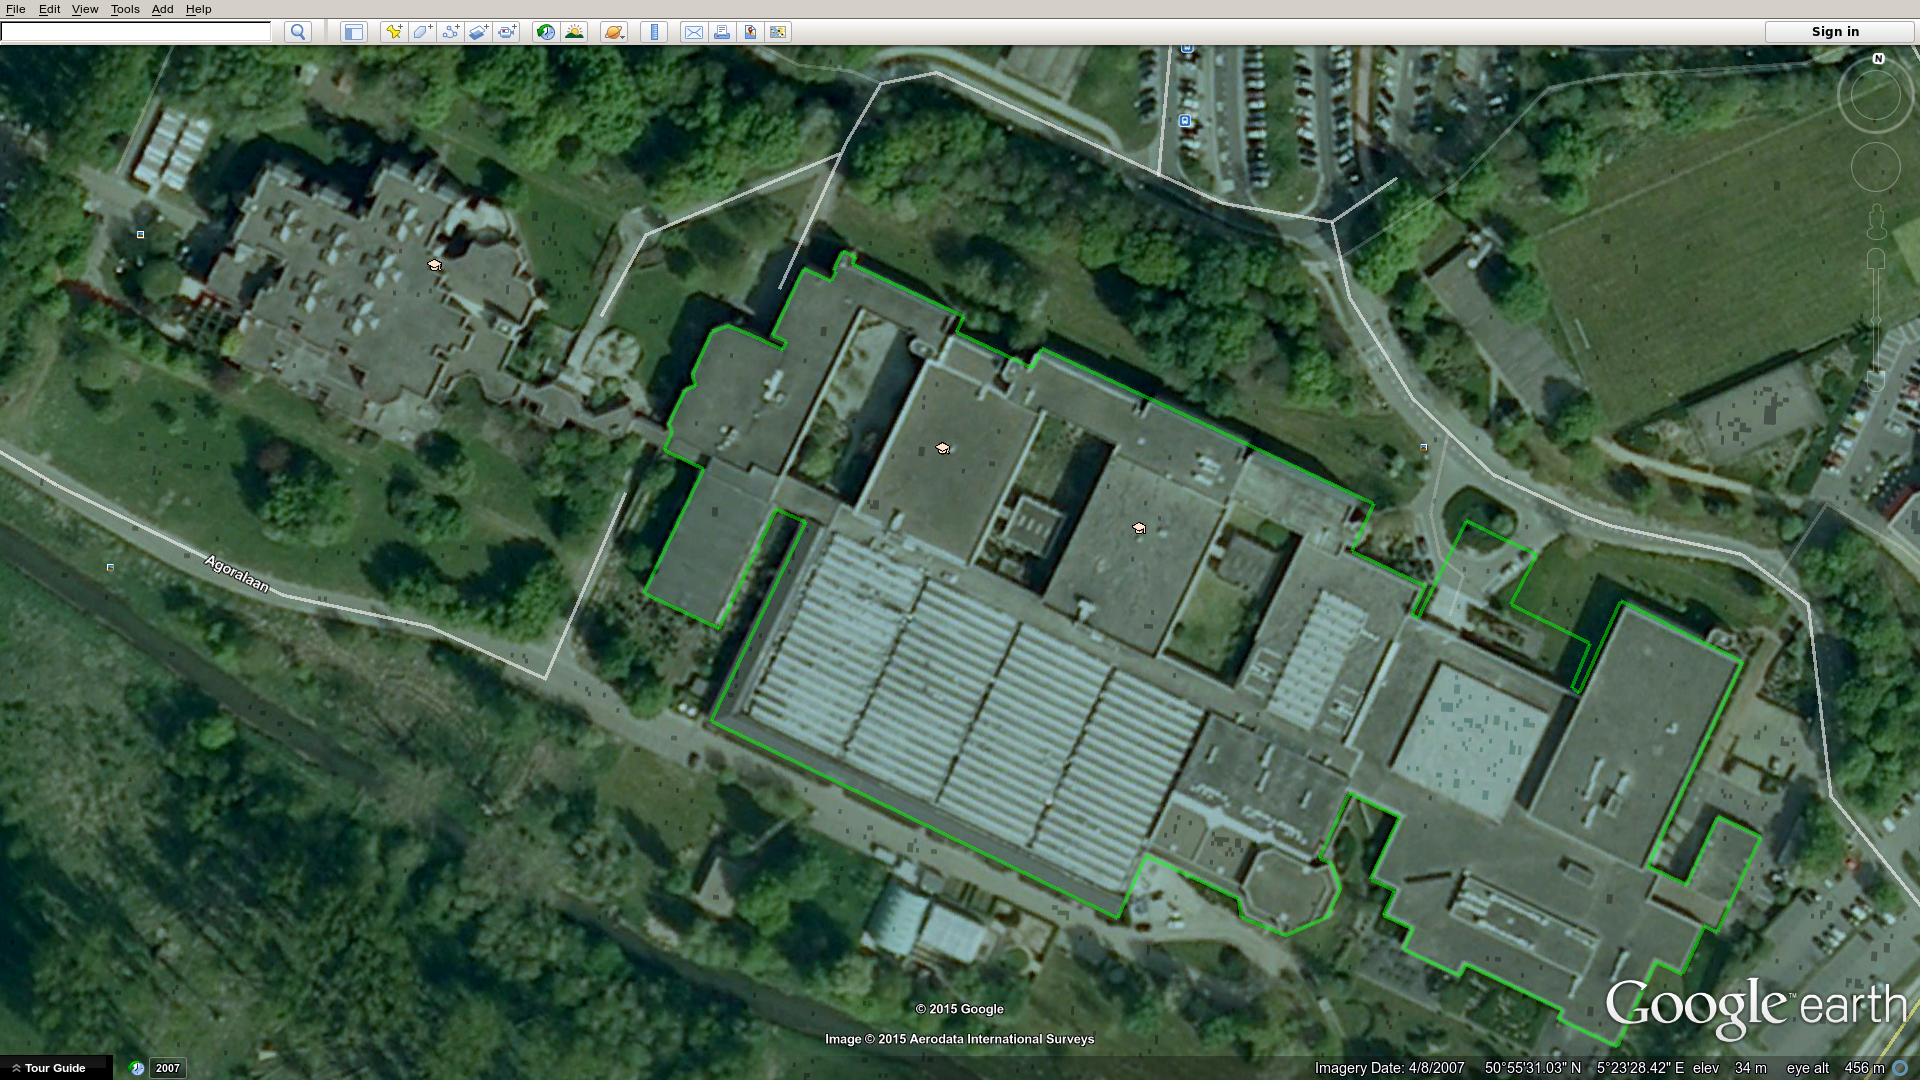
\includegraphics[width=\textwidth]{university_half}}
\end{frame}

\begin{frame}
  \frametitle{Inkonsistenz \hfill Lösung Nr. 18}
  \Wider{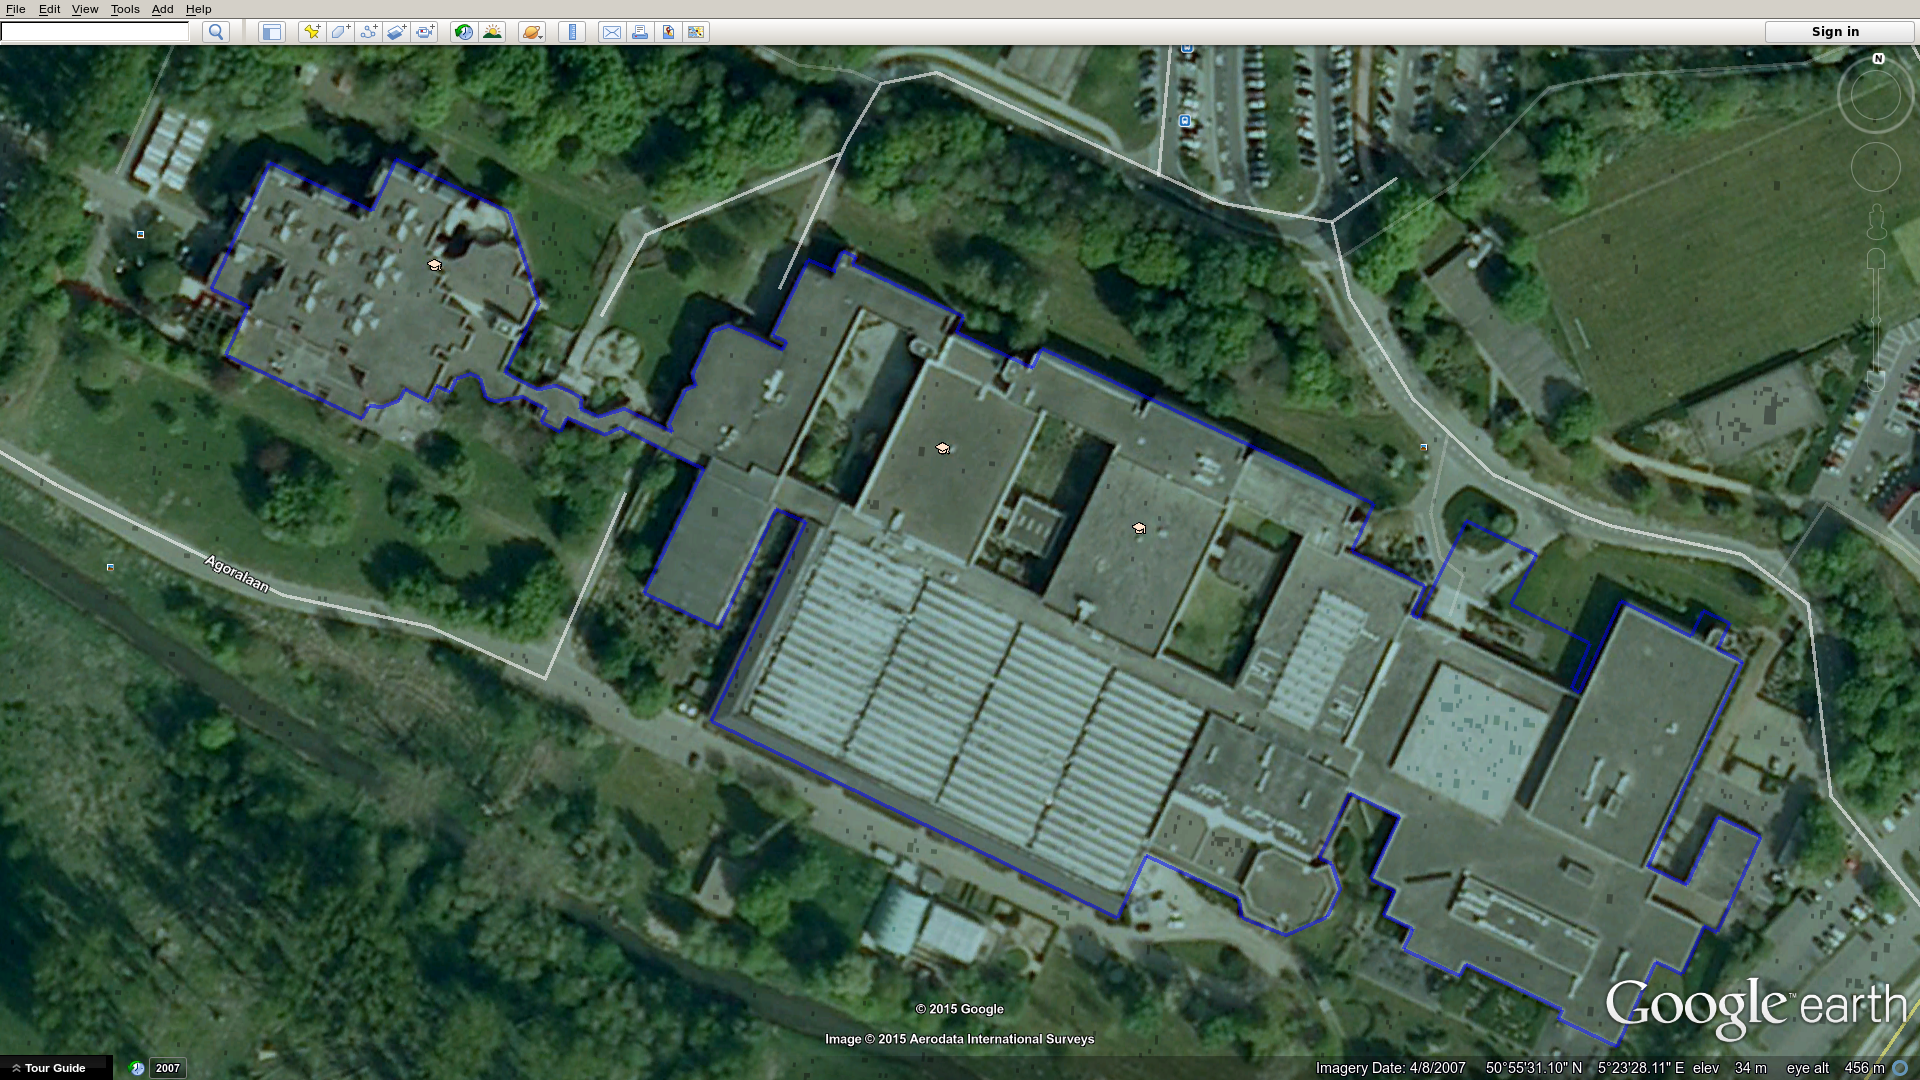
\includegraphics[width=\textwidth]{university_full}}
\end{frame}

\begin{frame}
  \frametitle{Inkonsistenz \hfill Lösung Nr. 16 \& 18}
  \Wider{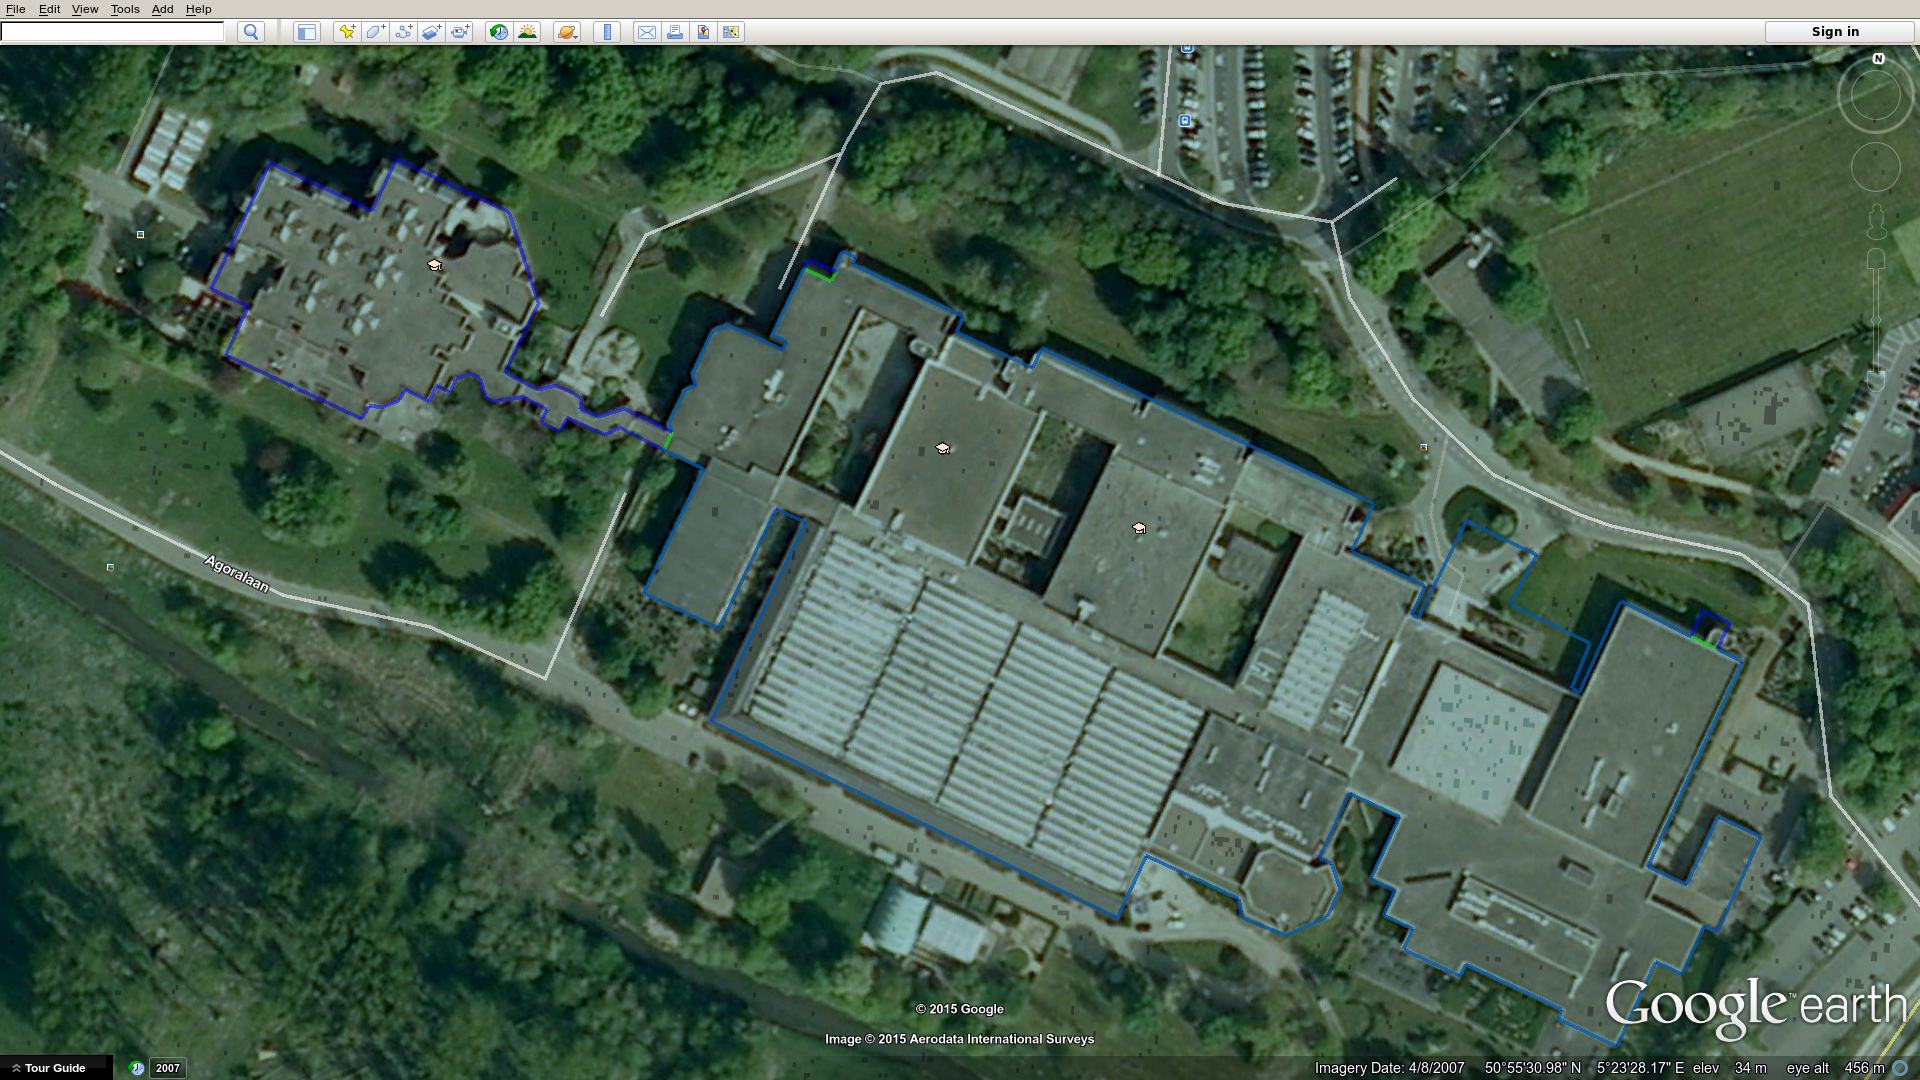
\includegraphics[width=\textwidth]{university_combine}}
\end{frame}

%%%%%%%%%%%%%%%%%%%%%%%%%%%%%%%%%%%%%%%%%%%%%%%%%%%%%%%%%%%%%%%%%%%%%%%%%%%%%%%%
% Bilder noch mal neu machen mit dickerer Strichbreite
%%%%%%%%%%%%%%%%%%%%%%%%%%%%%%%%%%%%%%%%%%%%%%%%%%%%%%%%%%%%%%%%%%%%%%%%%%%%%%%%
\begin{frame}
  \frametitle{Unvollständige Datensätze \hfill Nr. 38}
  \Wider{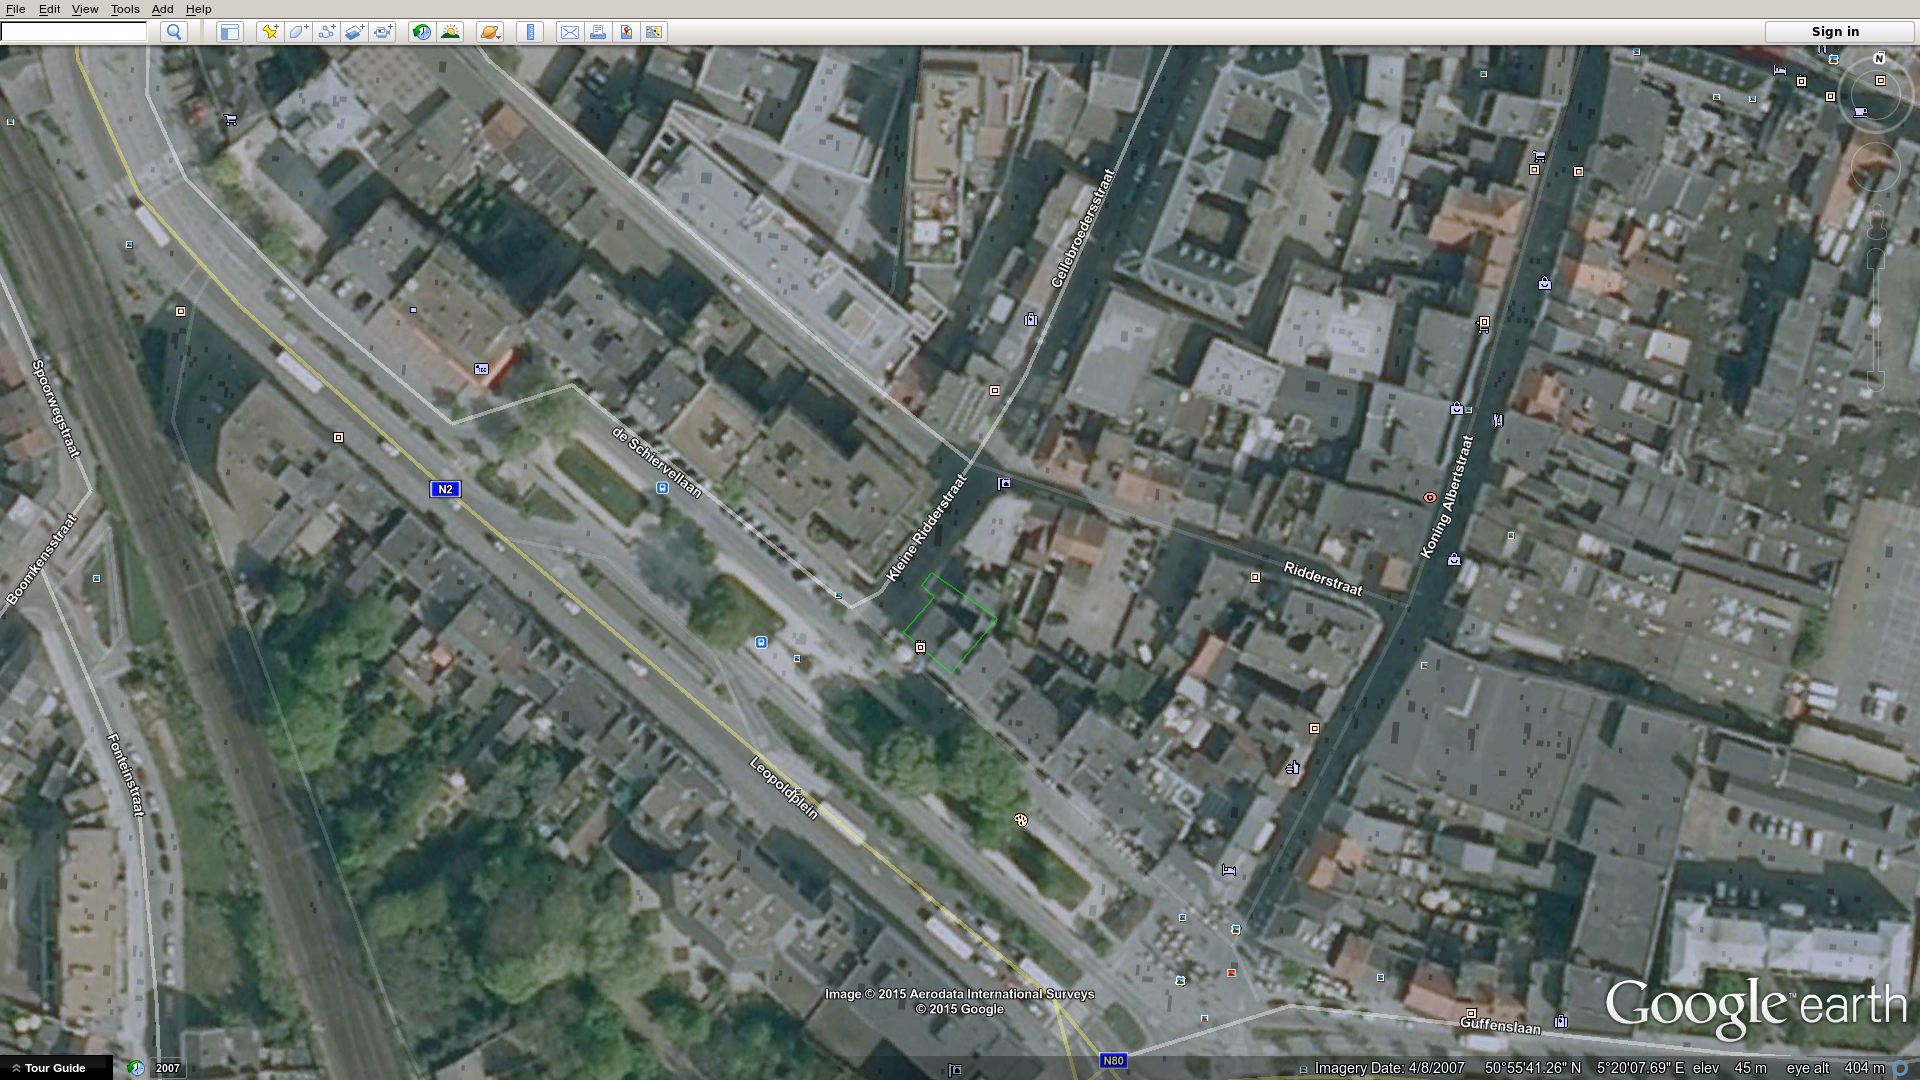
\includegraphics[width=\textwidth]{google_earth}}
\end{frame}

\begin{frame}
  \frametitle{Unvollständige Datensätze \hfill Nr. 38}
  \Wider{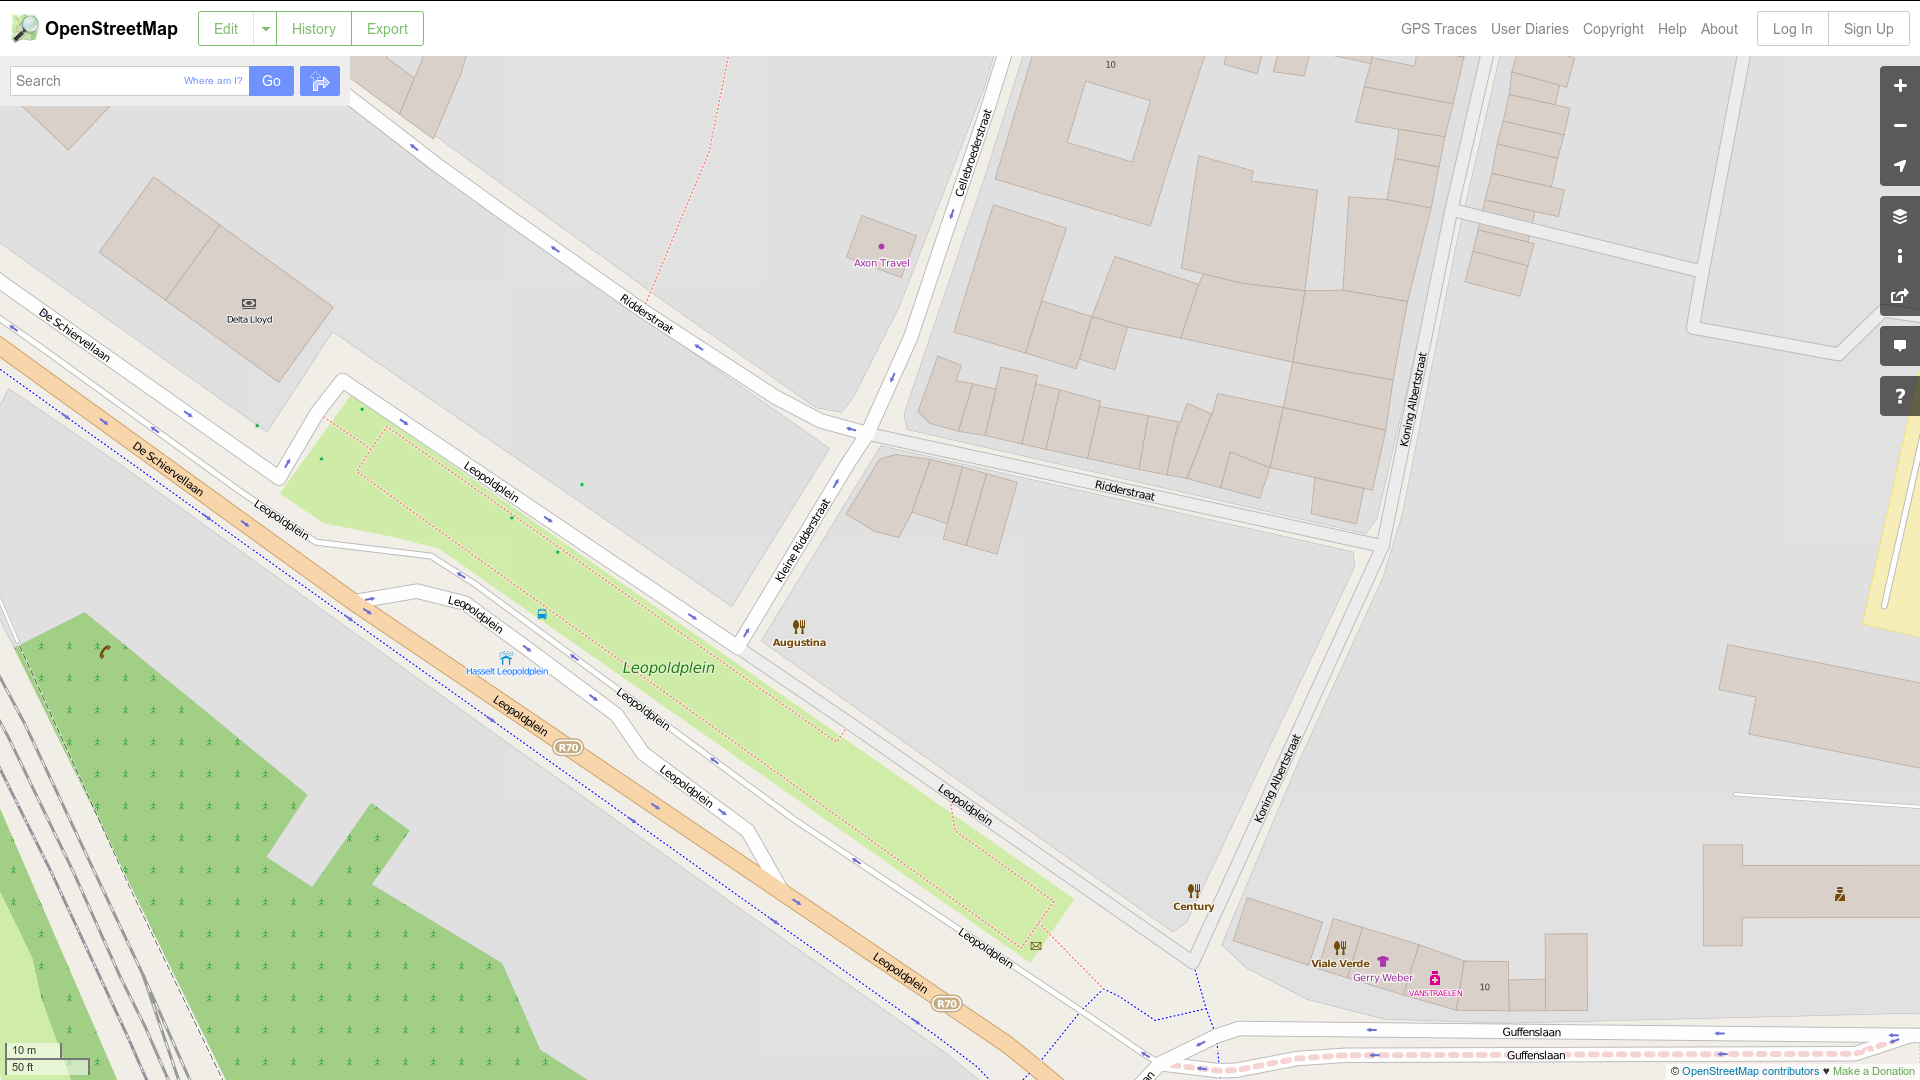
\includegraphics[width=\textwidth]{unvollstaendig}}
\end{frame}


%%%%%%%%%%%%%%%%%%%%%%%%%%%%%%%%%%%%%%%%%%%%%%%%%%%%%%%%%%%%%%%%%%%%%%%%%%%%%%%%
% Auch dickere Strichbreite
%%%%%%%%%%%%%%%%%%%%%%%%%%%%%%%%%%%%%%%%%%%%%%%%%%%%%%%%%%%%%%%%%%%%%%%%%%%%%%%%
\begin{frame}
  \frametitle{Falsche Datensätze \hfill Nr. 40}
  \Wider{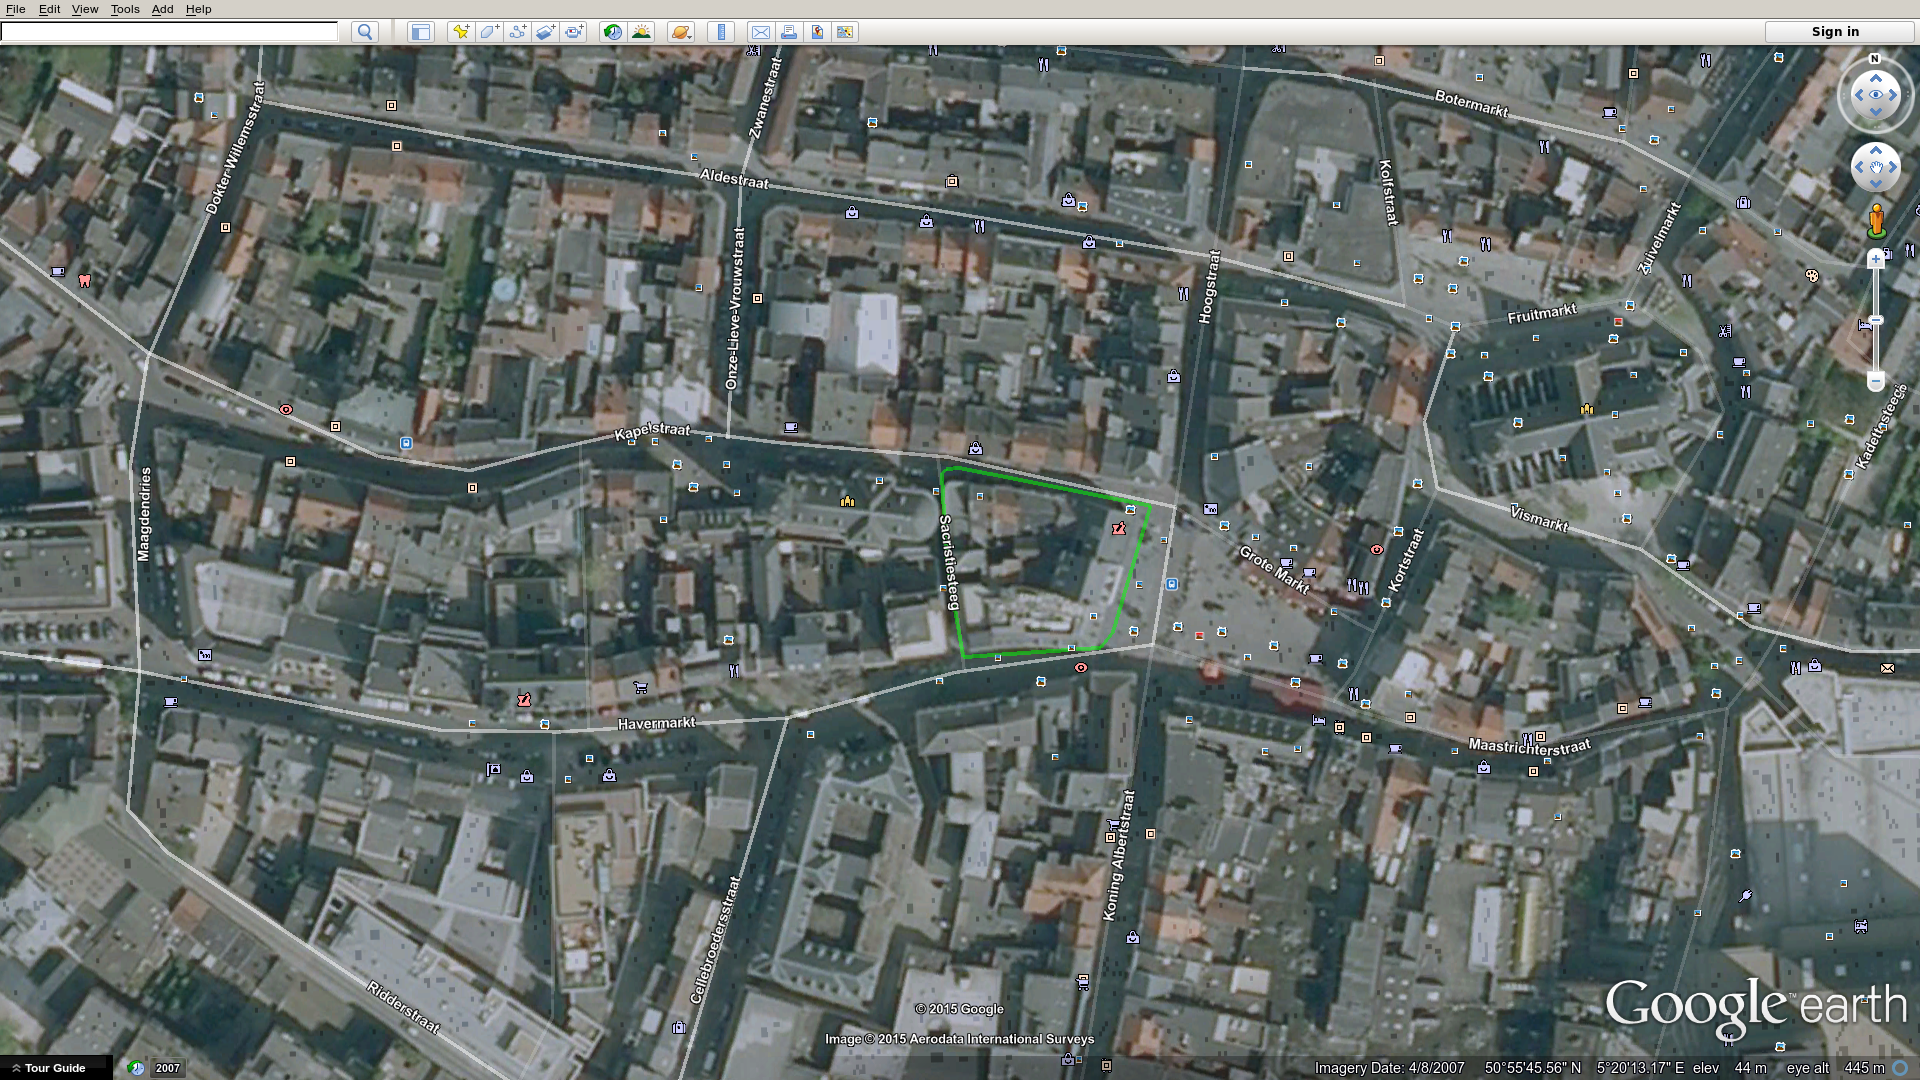
\includegraphics[width=\textwidth]{40_fail_earth}}
\end{frame}

\begin{frame}
  \frametitle{Falsche Datensätze \hfill Nr. 40}
  \Wider{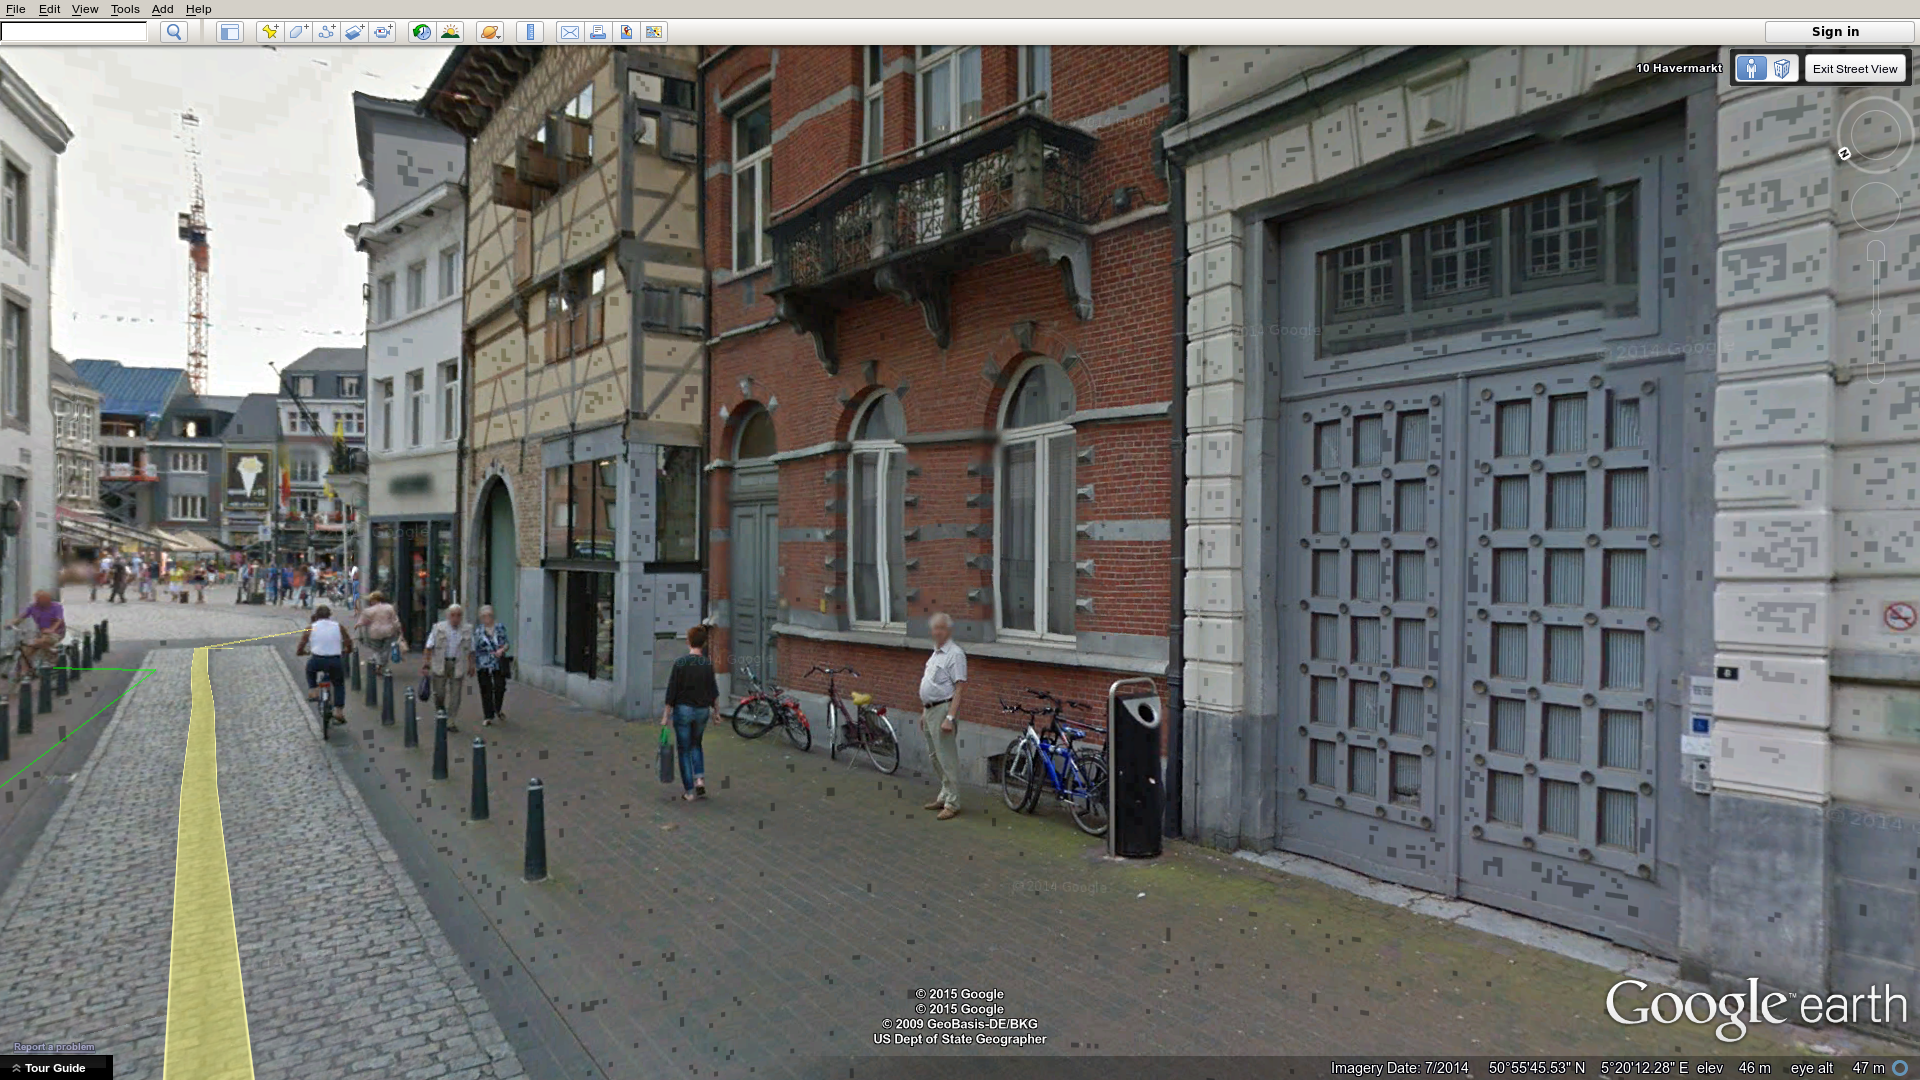
\includegraphics[width=\textwidth]{40_fail_street}}
\end{frame}

\begin{frame}
  \frametitle{Falsche Datensätze \hfill Nr. 40}
  \Wider{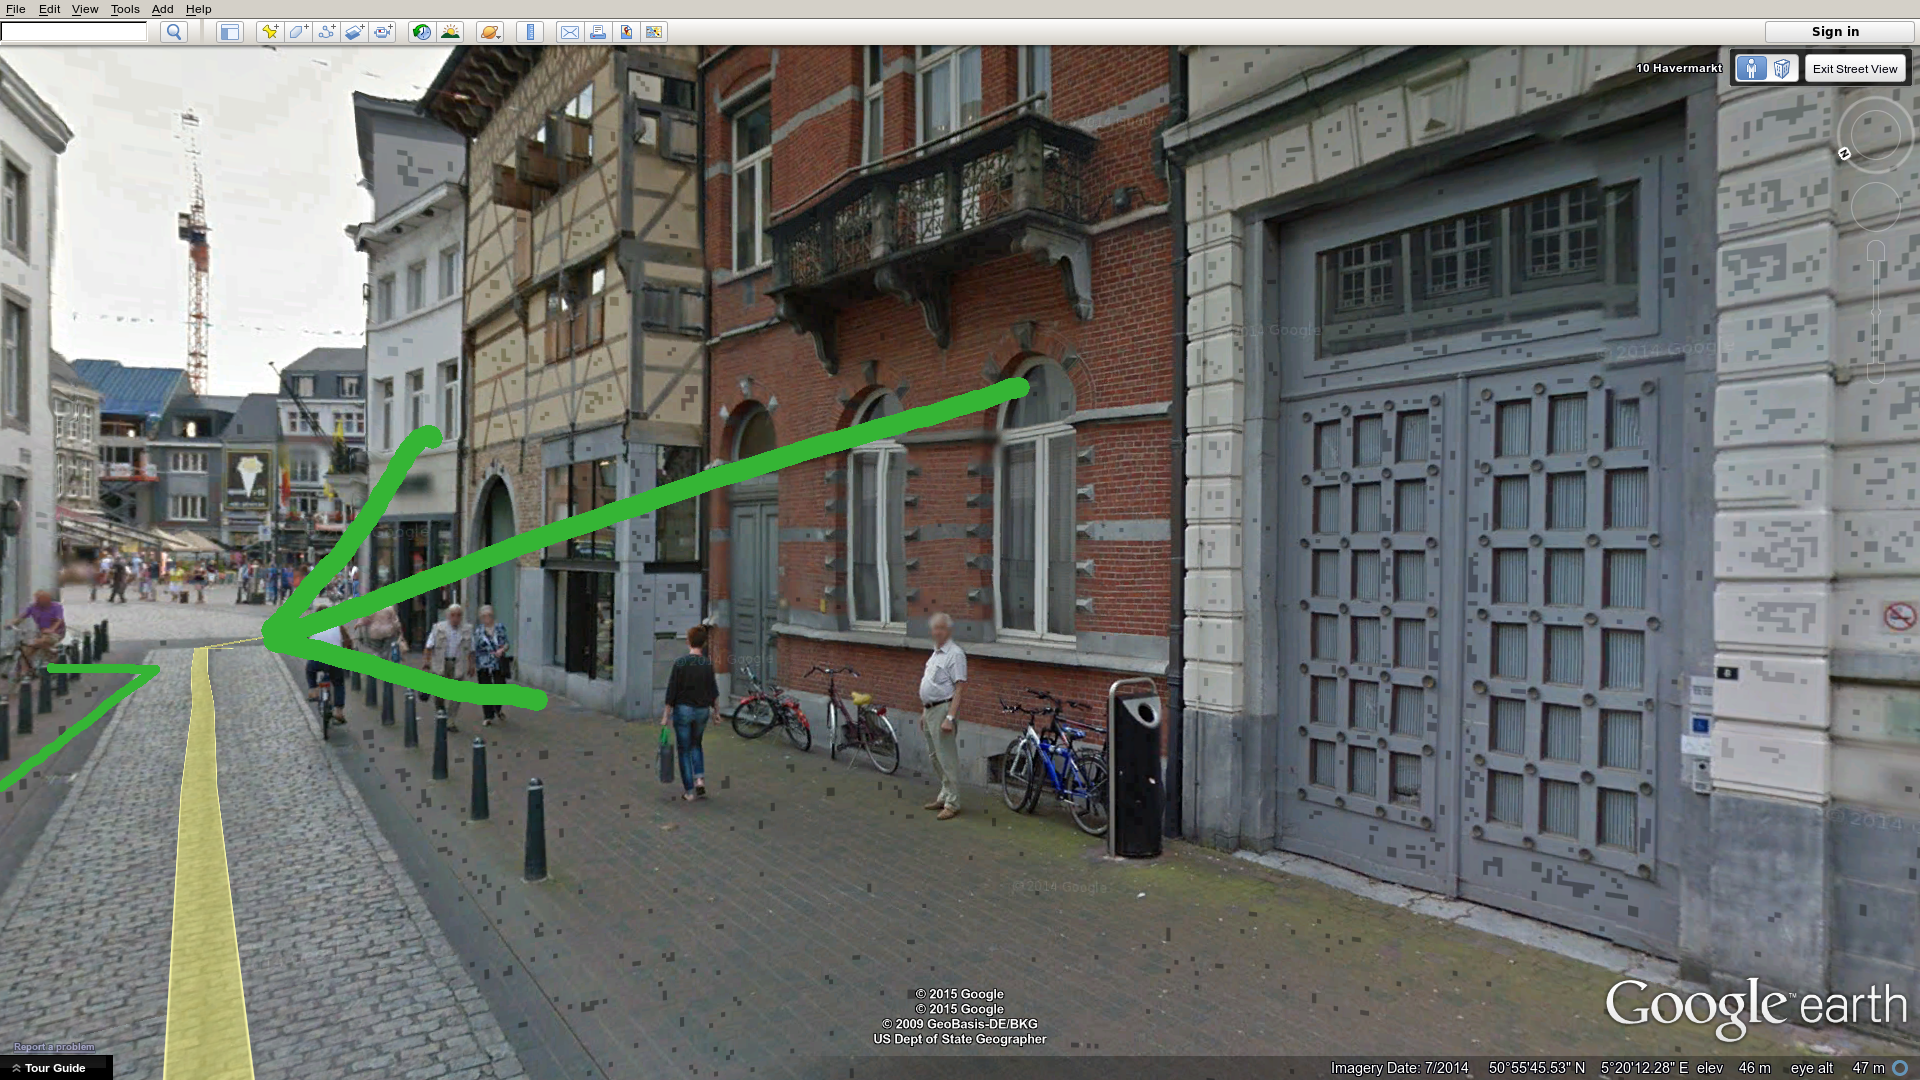
\includegraphics[width=\textwidth]{40_fail_street_building}}
\end{frame}

\begin{frame}
  \frametitle{Falsche Datensätze \hfill Nr. 40}
  \Wider{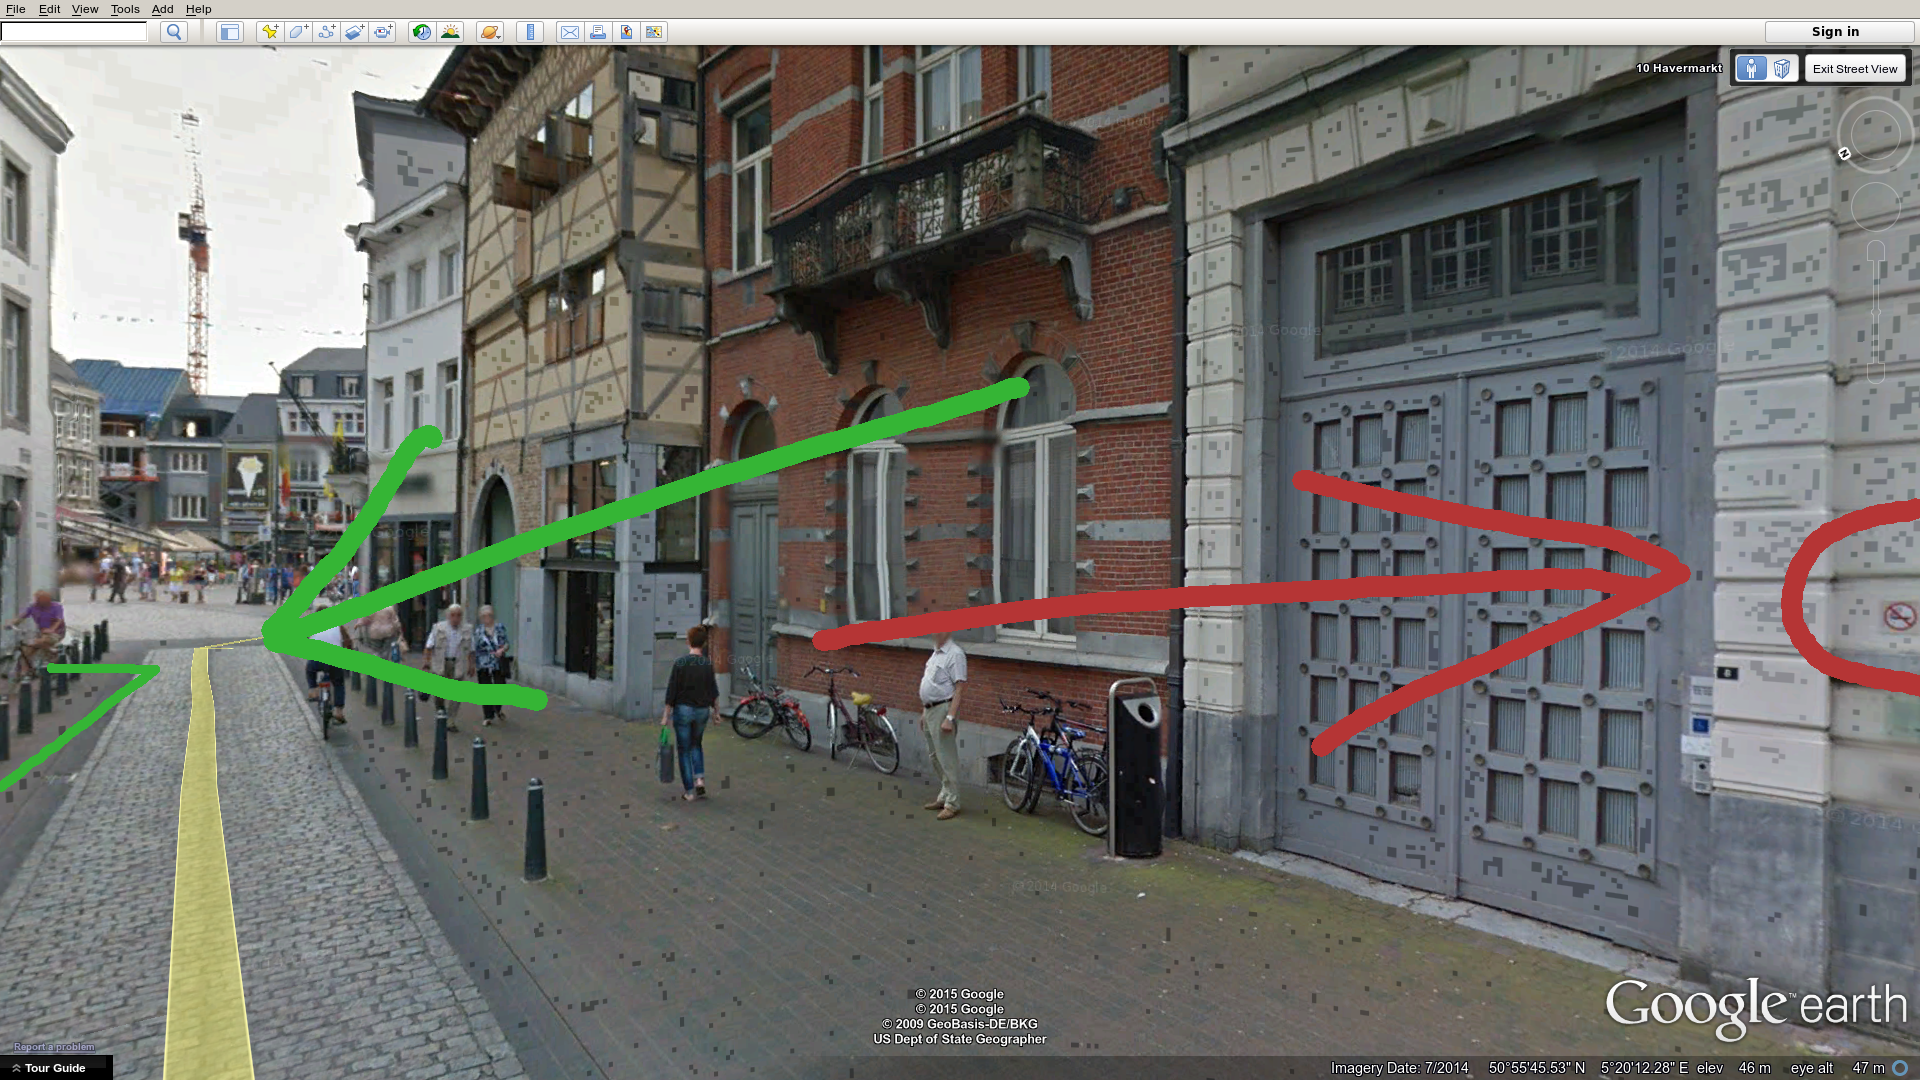
\includegraphics[width=\textwidth]{40_fail_street_sign}}
\end{frame}

%\begin{frame}
%  \frametitle{Falsche Datensätze \hfill Nr. 40}
%  \Wider{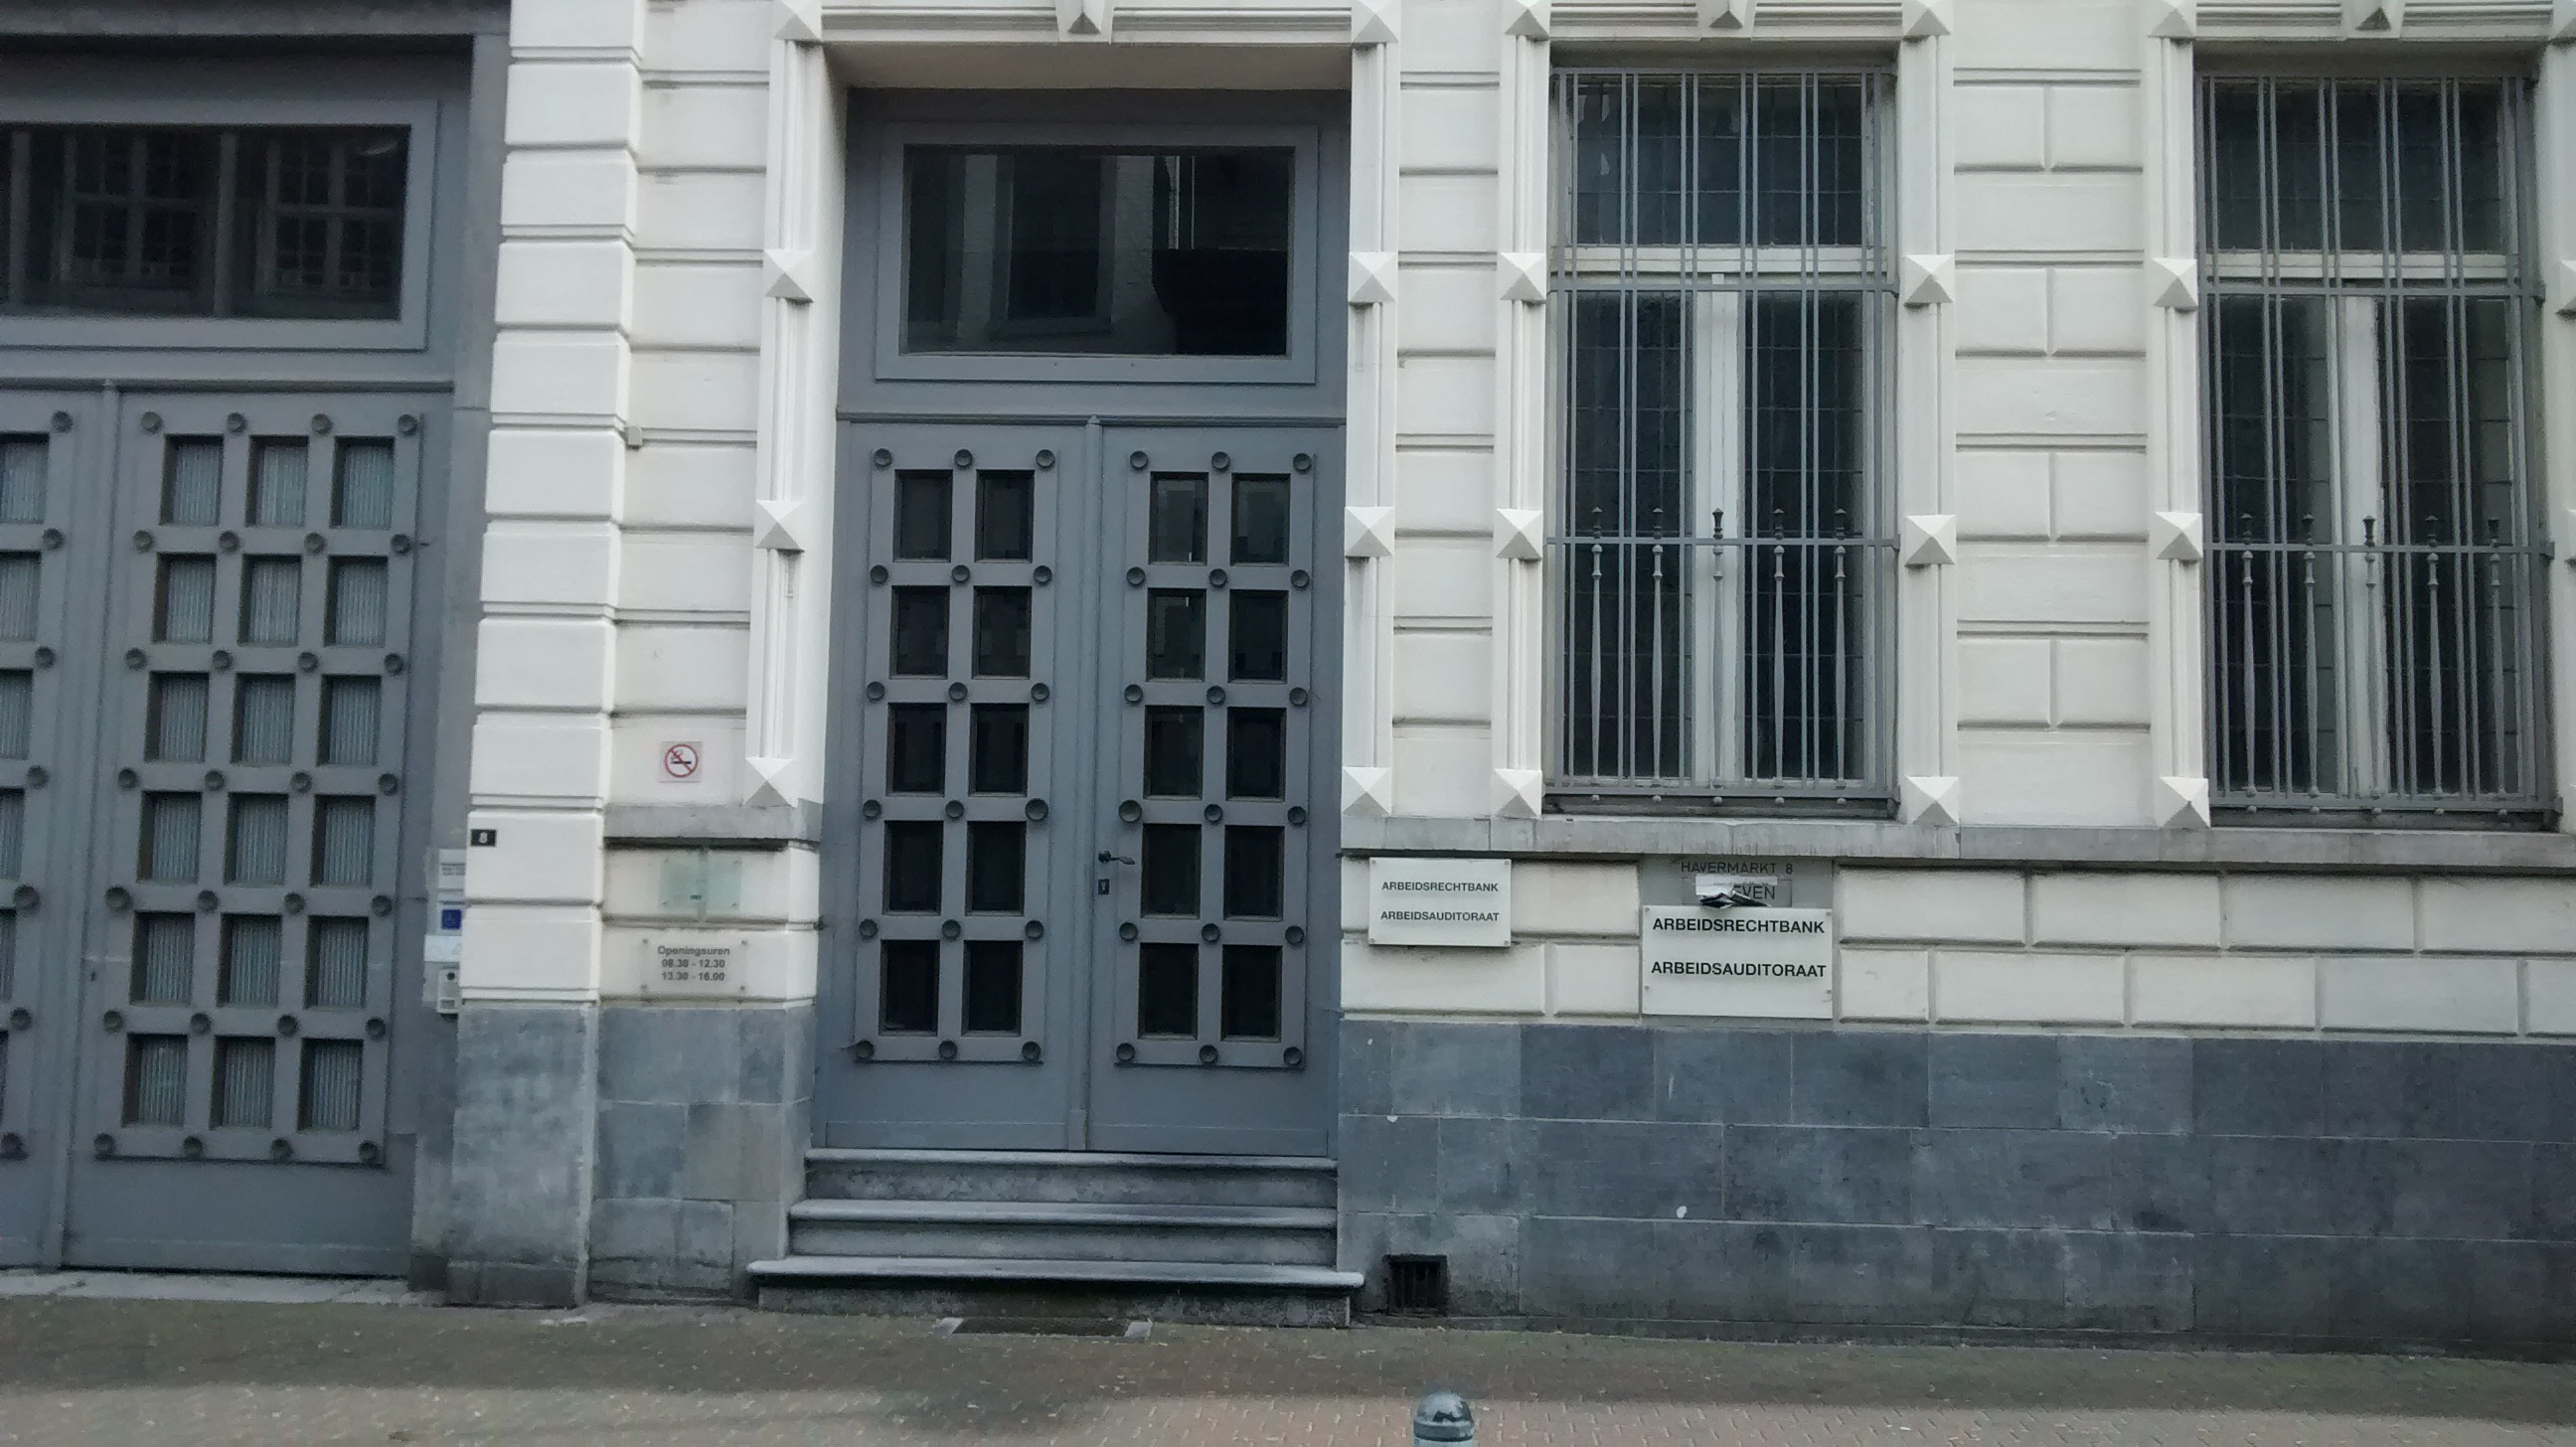
\includegraphics[width=\textwidth]{0040}}
%\end{frame}


%%%%%%%%%%%%%%%%%%%%%%%%%%%%%%%%%%%%%%%%%%%%%%%%%%%%%%%%%%%%%%%%%%%%%%%%%%%%%%%%
% Formatierung von dem hier verbessern!
%%%%%%%%%%%%%%%%%%%%%%%%%%%%%%%%%%%%%%%%%%%%%%%%%%%%%%%%%%%%%%%%%%%%%%%%%%%%%%%%
\begin{frame}
  \frametitle{3 Klassen}
\begin{columns}
  \begin{column}{0.33\textwidth}
  Einfache Datensätze
  \begin{itemize}
  \item 1 - 15
  \item 17 - 32
  \item 35
  \item 37
  \item 42
  \item 46 - 48
  \item 52
  \item 54
  \item 63 - 83
  \item 86 - 89
  \item 91 - 92
  \item 94 - 95
  \end{itemize}
  \end{column}
    \begin{column}{0.33\textwidth}
    Unvollständige Datensätze
    \begin{itemize}
    \item 33 - 34
    \item 36
    \item 38
    \item 39
    \item 41
    \item 43 - 45
    \item 49 - 50
    \item 55 - 62
    \end{itemize}
    \end{column}
  \begin{column}{0.33\textwidth}
  Schwere Datensätze
  \begin{itemize}
  \item 16
  \item 33
  \item 40
  \item 43
  \item 51
  \item 57
  \item 59
  \item 62
  \item 84
  \item 85
  \item 90
  \item 93
  \item 96
  \end{itemize}
  \end{column}
\end{columns}
\end{frame}
